%%%% ijcai22.tex
\RequirePackage{luatex85}
\typeout{IJCAI--22 Instructions for Authors}

% These are the instructions for authors for IJCAI-22.

\documentclass{article}
\pdfpagewidth=8.5in
\pdfpageheight=11in
% The file ijcai22.sty is NOT the same as previous years'
\usepackage{ijcai22}

% Use the postscript times font!
\usepackage{times}
\usepackage{soul}
\usepackage{url}
\usepackage[hidelinks]{hyperref}
\usepackage[utf8]{inputenc}
\usepackage[small]{caption}
\usepackage{graphicx}
\usepackage{amsmath}
\usepackage{amsthm}
\usepackage{booktabs}
\usepackage{algorithm}
\usepackage{algorithmic}
\urlstyle{same}

% the following package is optional:
%\usepackage{latexsym}

% See https://www.overleaf.com/learn/latex/theorems_and_proofs
% for a nice explanation of how to define new theorems, but keep
% in mind that the amsthm package is already included in this
% template and that you must *not* alter the styling.
\newtheorem{example}{Example}
\newtheorem{theorem}{Theorem}

% Following comment is from ijcai97-submit.tex:
% The preparation of these files was supported by Schlumberger Palo Alto
% Research, AT\&T Bell Laboratories, and Morgan Kaufmann Publishers.
% Shirley Jowell, of Morgan Kaufmann Publishers, and Peter F.
% Patel-Schneider, of AT\&T Bell Laboratories collaborated on their
% preparation.

% These instructions can be modified and used in other conferences as long
% as credit to the authors and supporting agencies is retained, this notice
% is not changed, and further modification or reuse is not restricted.
% Neither Shirley Jowell nor Peter F. Patel-Schneider can be listed as
% contacts for providing assistance without their prior permission.

% To use for other conferences, change references to files and the
% conference appropriate and use other authors, contacts, publishers, and
% organizations.
% Also change the deadline and address for returning papers and the length and
% page charge instructions.
% Put where the files are available in the appropriate places.

% PDF Info Is REQUIRED.
% Please **do not** include Title and Author information
\pdfinfo{
/TemplateVersion (IJCAI.2022.0)
}

\title{Sequence Is All You Need For Accurate RNA-Distance Prediction}

% Single author syntax
\author{
    Author Name
    \affiliations
    Affiliation
    \emails
    pcchair@ijcai-22.org
}

% Multiple author syntax (remove the single-author syntax above and the \iffalse ... \fi here)
% Check the ijcai22-multiauthor.tex file for detailed instructions
\iffalse
\author{
First Author$^1$
\and
Second Author$^2$\and
Third Author$^{2,3}$\And
Fourth Author$^4$
\affiliations
$^1$First Affiliation\\
$^2$Second Affiliation\\
$^3$Third Affiliation\\
$^4$Fourth Affiliation
\emails
\{first, second\}@example.com,
third@other.example.com,
fourth@example.com
}
\fi

\begin{document}

\maketitle

\begin{abstract}
      Many biological tasks have been well tackled with data accumulation and machine learning advances, particularly protein-related research. However, RNA structure prediction remains a significant challenge in the field due to RNA data limitations. To offer accurate forecasts of RNA 3D-structure, we propose such a task in defining the distance of arbitrary bases in the RNA primary sequence. This regression task is more informative to subsequent 3D folding methods but more complicated than the well-known RNA secondary structure prediction. 

In this work, we reveal that with only primary sequential information, we can gain accurate inferences on RNA bases' distance with a sizeable pre-trained RNA language model and a well-designed downstream transformer followed by a unrolled constraint layer. Our experiments show that we outperform all convolutional-based models by a preferably big gap while obtaining rather good statistical results. Moreover, we also acquired a comparable performance with other methods at the contact forecast level by degrading our distance prediction output. Moreover, our approach unified the view of language modeling and distance regression, a new perspective by viewing each predicted embedding as a column vector of the decomposed distance matrix. Our framework will foreseeably be a good guidance for 3D-structure prediction.

\end{abstract}
\section{Introduction}
  \input{introduction.tex}
\section{Methodology}
  The whole framework could be mainly divided into four stages, lan pre-training , DiT pre-training, distance map training, and finally the inference stage.


In order to achieve accurate RNA-Distance predictions from vanilla Sequence


%\subsection{Se}

\subsection{RNA-FM Pre-Training}

The intention of this pre-training stage aims to provide rich RNA sequence representations for further downstream tasks as prescribed. A Bert-based language model with 12 transformer encoder blocks \cite{devlin2018bert} was trained on around 26 million non-coding RNA sequences in an unsupervised manner, where details could be found via another work [*]. After the training stage, a learned embedding layer will map an RNA sequence of Length $L$  to a $L\times 640$ tensor.

Noticed that this trained RNA Bert model could be applied directly for fine-tuning in other tasks. However, the difficulty of such an approach lies in the gap between enormous model capacity and relatively small downstream datasets. Thus, we reimplement a transformer-based downstream model DiT specified for tackling the distance prediction task.

\subsection{DiT pre-training}

F

\subsection{Distance Map Tuning}
DiT pre-training enbales 


\begin{figure*}[]
    \begin{center}
    %\caption{}\label{fig1}
    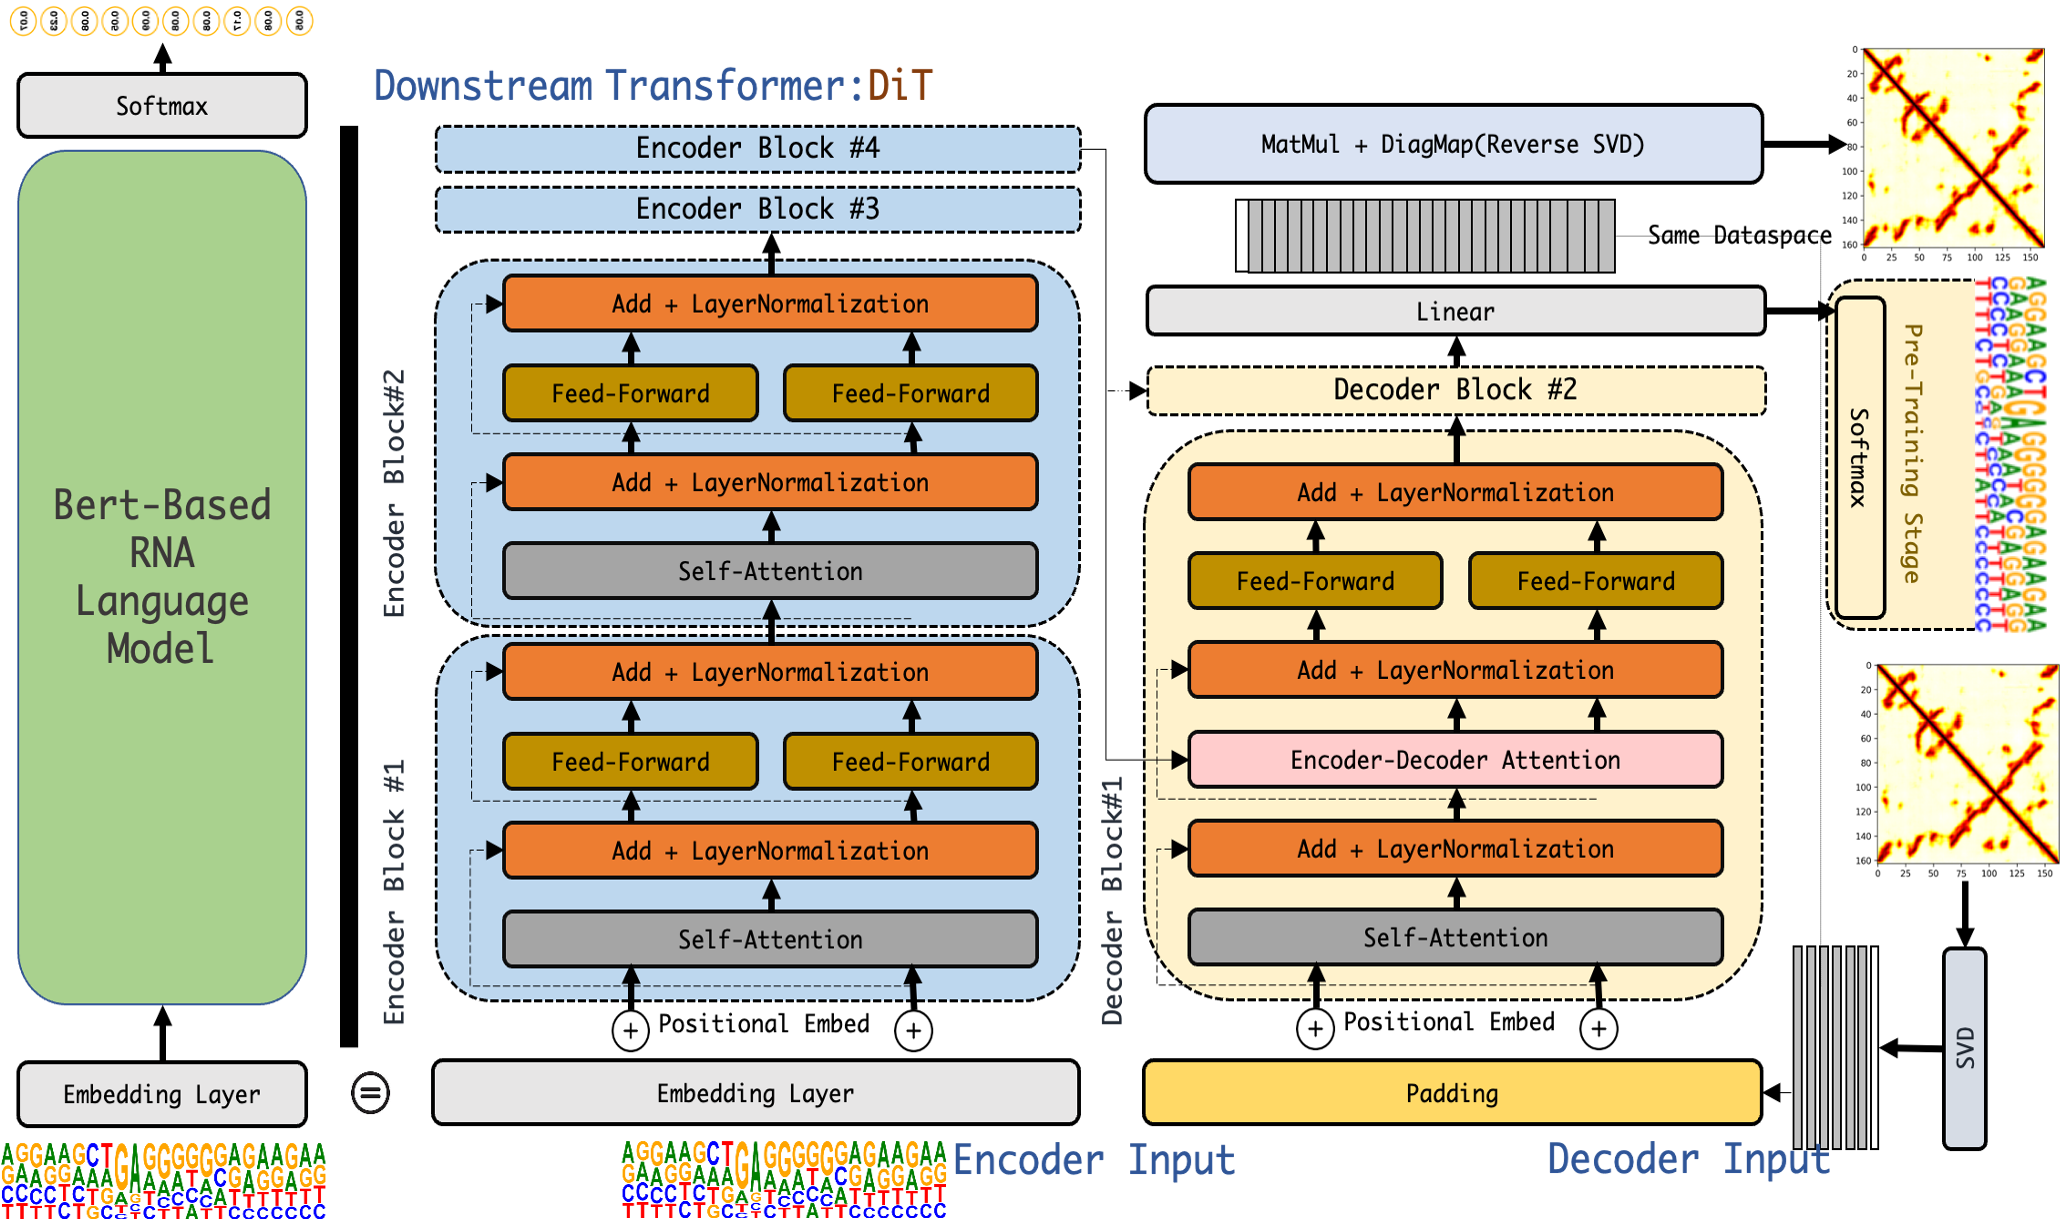
\includegraphics[width=1.0\textwidth]{1.png}
    \caption{Overview of the model's traininaag Stage}\label{Trainig Stage}
    \end{center}
\end{figure*}

\begin{figure*}[]
    \begin{center}
    %\caption{}\label{fig1}
    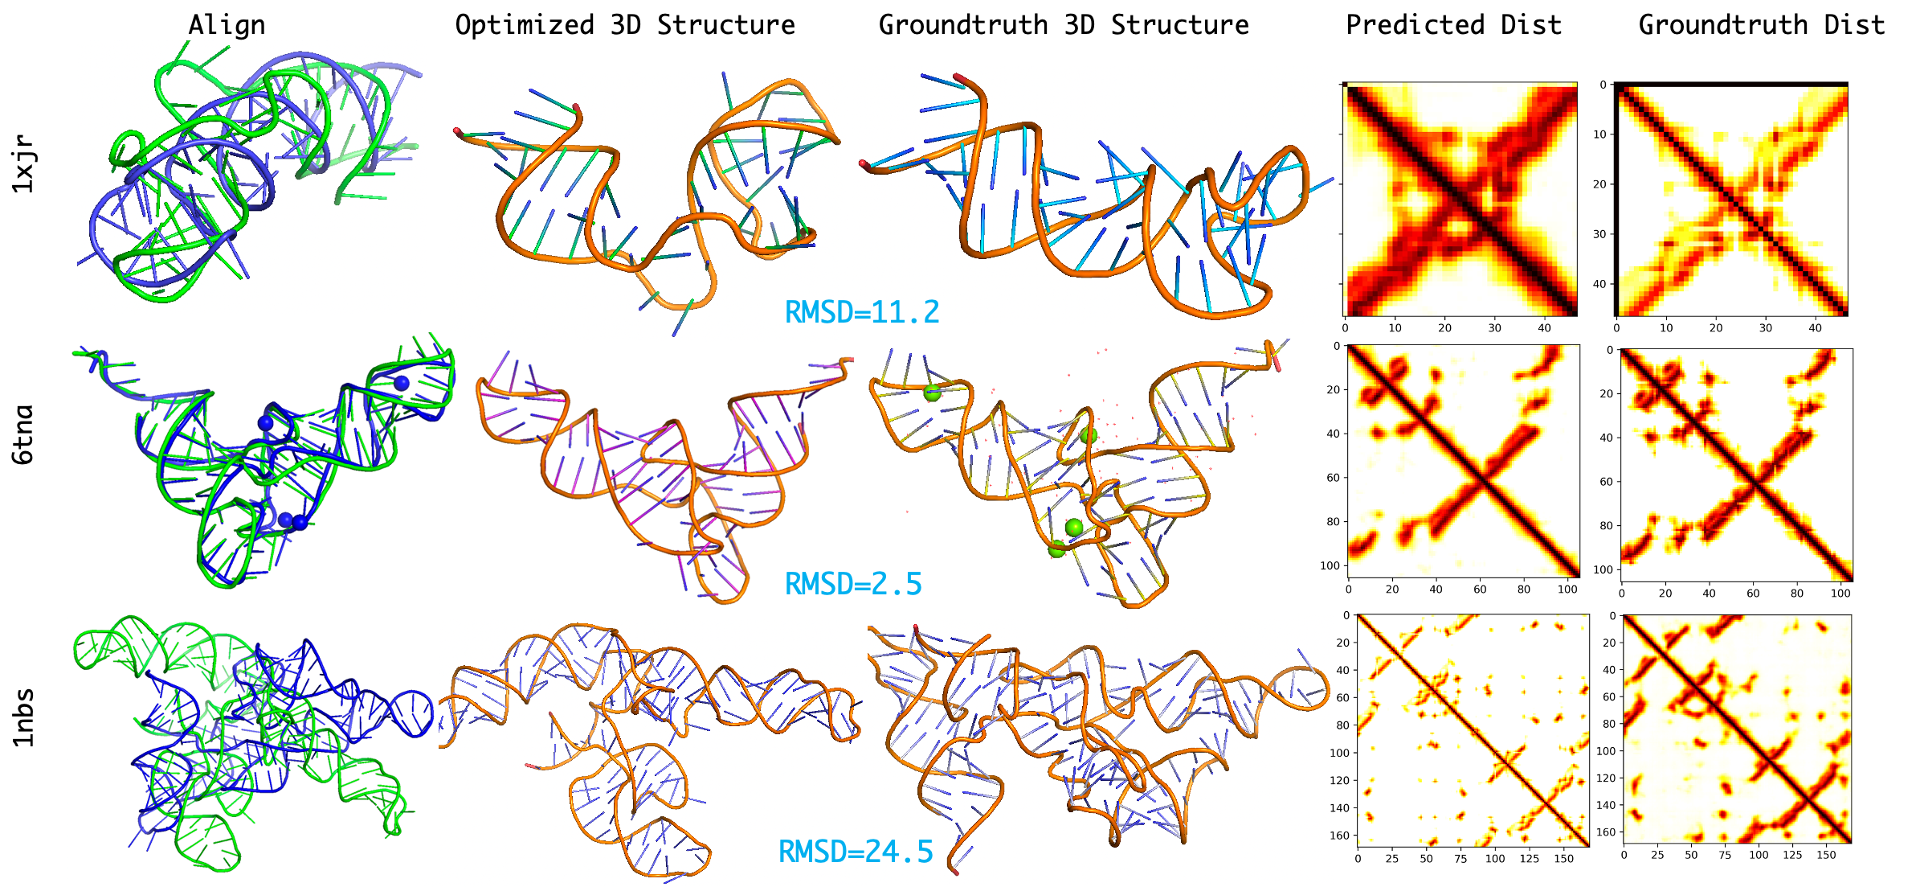
\includegraphics[width=1.0\textwidth]{2.png}
    \caption{Overview of the model'as training Stage}\label{Trainig Stage}
    \end{center}
\end{figure*}

\begin{figure*}[]
    \begin{center}
    %\caption{}\label{fig1}
    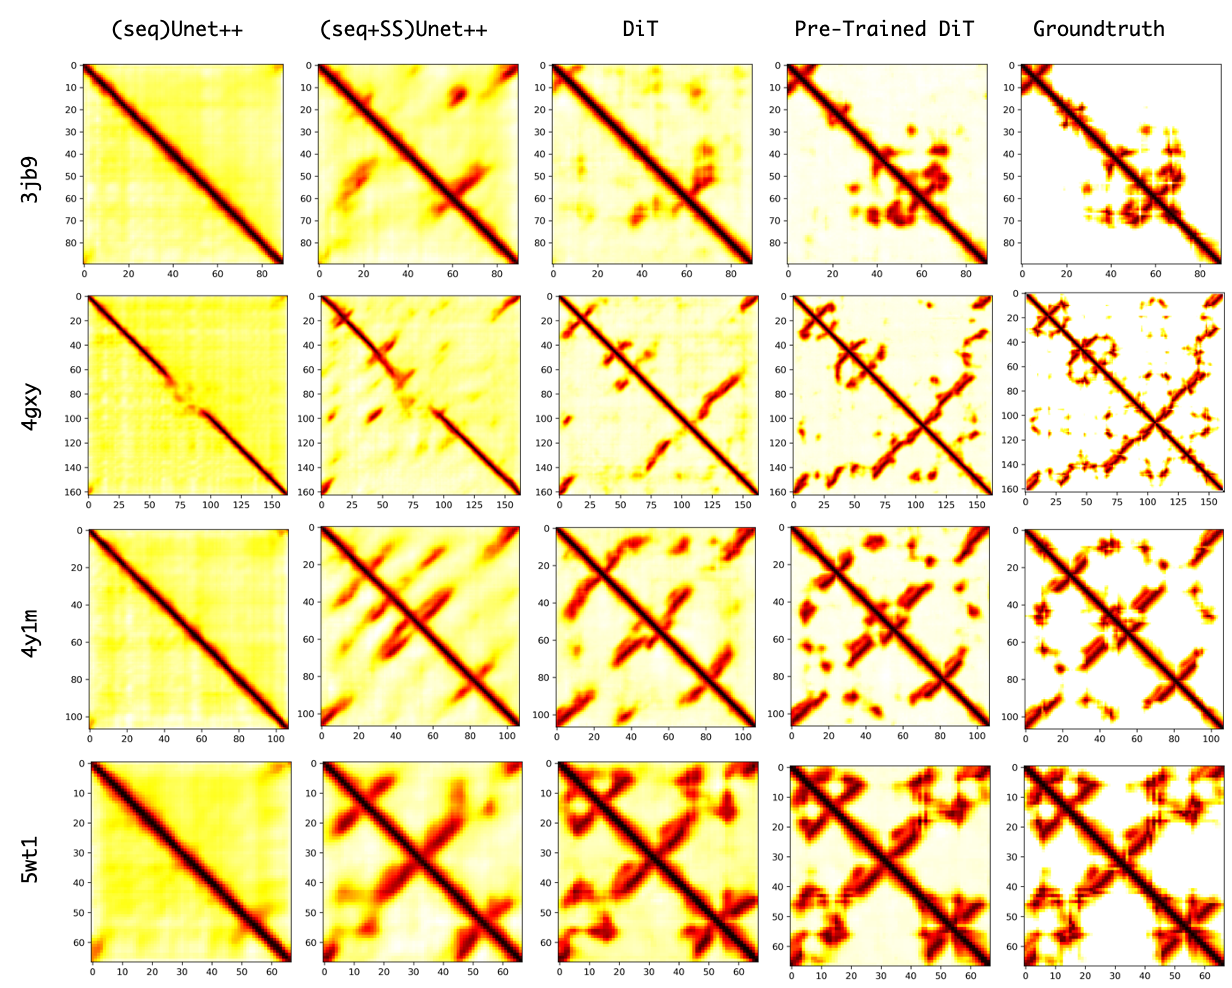
\includegraphics[width=0.8\textwidth]{3.png}
    \caption{Overview of the modelas's training Stage}\label{Trainig Stage}
    \end{center}
\end{figure*}
\begin{figure}[]
    \begin{center}
    %\caption{}\label{fig1}
    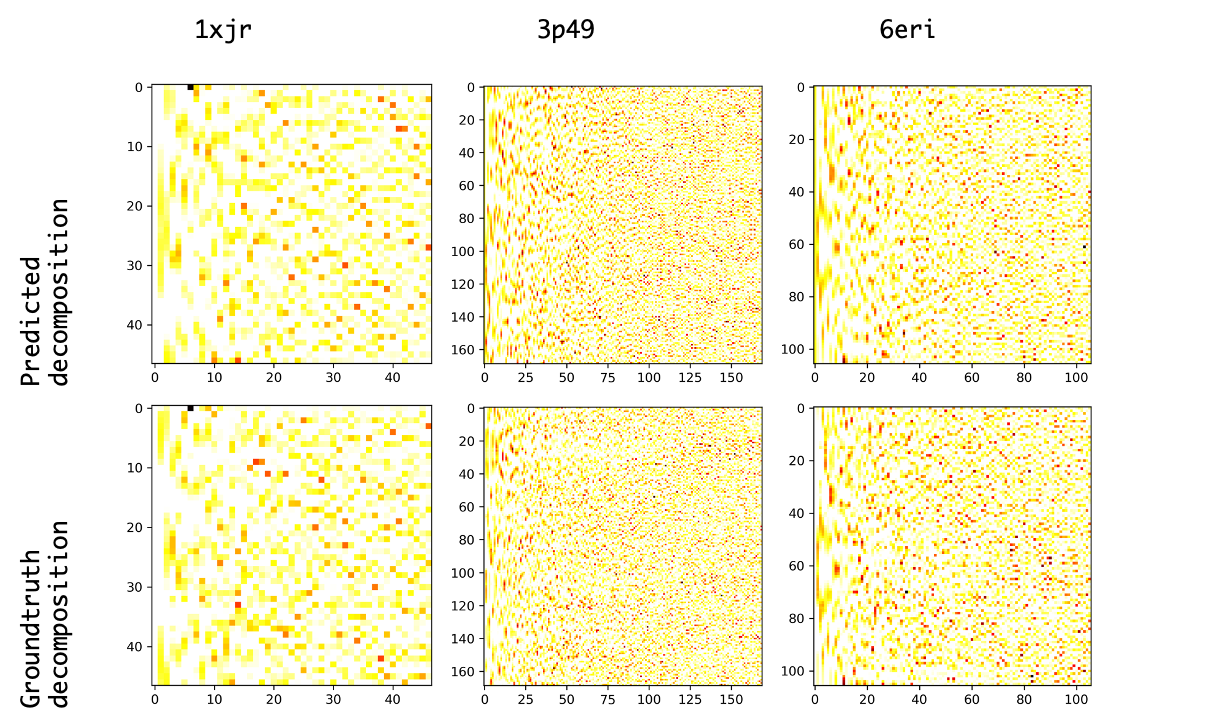
\includegraphics[width=0.5\textwidth]{svg.png}
    \caption{Overview of the modelas's training Stage}\label{Trainig Stage}
    \end{center}
\end{figure}
\begin{figure*}[]
    \begin{center}
    %\caption{}\label{fig1}
    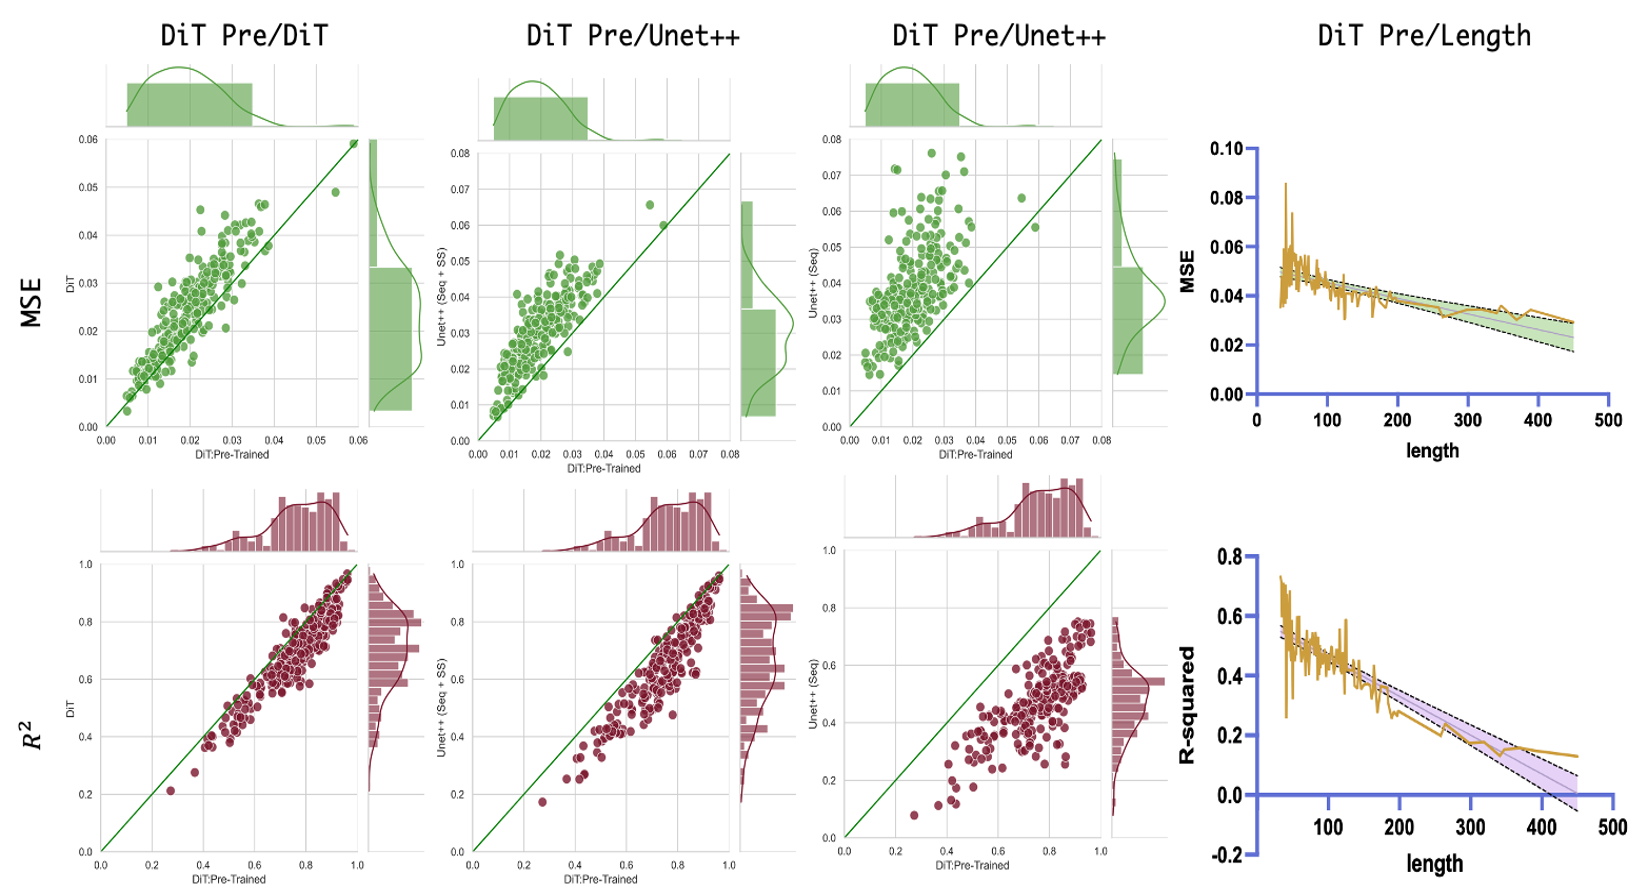
\includegraphics[width=1.0\textwidth]{4.png}
    \caption{Overview of the model's traiaaaaning Stage}\label{Trainig Stage}
    \end{center}
\end{figure*}



\section{Methodology}
\section{Results}
  \input{results.tex}
\section{Results}
\section{Acknowledgement}
  \input{acknowledgement.tex}
\section{Acknowledgement}

The {\it IJCAI--22 Proceedings} will asdasdsads

%% The file named.bst is a bibliography style file for BibTeX 0.99c
\bibliographystyle{named}
\bibliography{ijcai22}

\end{document}

